% Revisão OK 12/10
\chapter{Rotas do back-end}

A seguir são listadas e explicadas todas as rotas públicas do backend. As
rotas de administração são explicadas na seção "Interface de Administração".

\section{Rota raiz}

Página inicial, apresenta a lista de aeródromos para que o usuário escolha um. 
Internamente, por meio do ORM, é feita a seleção dos campos \texttt{AerodromeName},
\texttt{ICAO} e \texttt{City} dos aeródromos com isPublished como verdadeiro e o
 resultado é posto em uma lista de tuplas que é enviada para o template.

Para um usuário logado também são mostrados os aeródromos não publicados.

Exemplo do resultado enviado à ferramenta de template:

\lstinputlisting[label=resp:root, title={Resposta da root}, caption={Resposta da root}, language=Python]{code/resp-root.json}


\section{Rota: /info/\{ICAO\}}

Retorna informações do aerodrómo e seu metar decodificado. A seguir um exemplo
de resultado enviado ao Jinja2.

\lstinputlisting[label=resp:root, title={Resposta da rota info}, caption={Resposta da rota info}, language=Python]{code/resp-info.json}


\section{Rota: /history/\{ICAO\}}
É uma página estática com os gráficos históricos para os doze últimos METARs.
Mais informações do capítulo "Plotagem do METAR Histórico".


\section{Rota: /taf/\{ICAO\}}
Retorna o próximo TAF válido para este aeródromo com a explicação de cada item.

Exemplo do resultado enviado à ferramenta de template para o aeroporto do Galeão.

\lstinputlisting[label=resp:root, title={Resposta da rota taf}, caption={Resposta da rota tag}, language=Python]{code/resp-taf.json}


Perceba que os grupos TEMPO e BECMG são agrupados para que no front-end o usuário 
possa exibir ou ocultar cada grupo. Conforme mostra a imagem abaixo.


\begin{figure}[ht]
    \begin{center}
    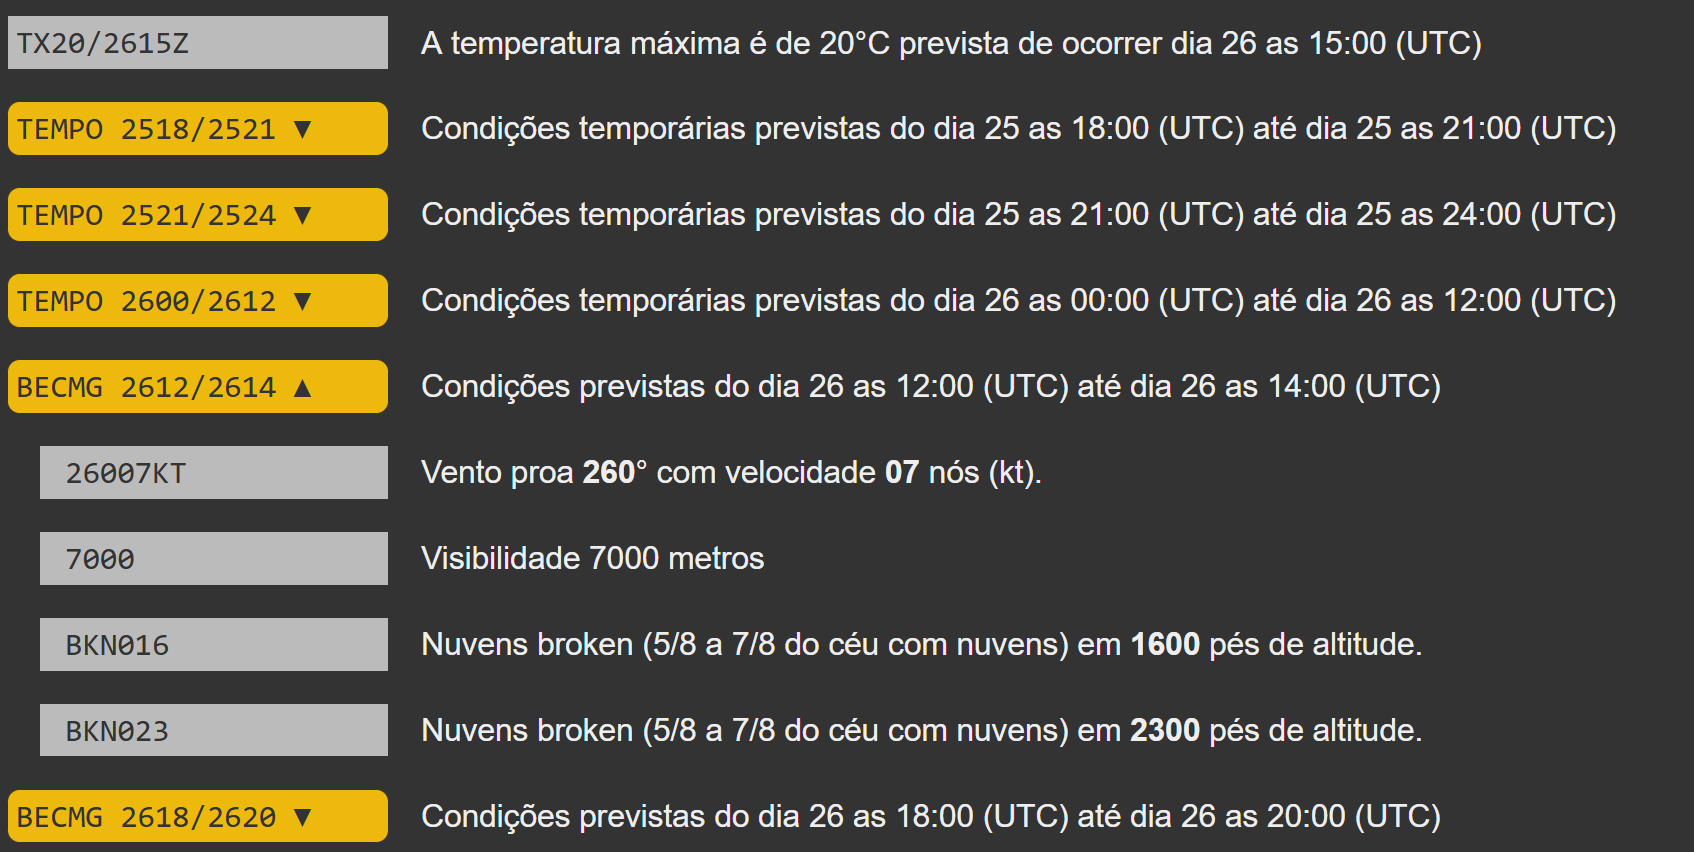
\includegraphics[width=400pt]{img/BECMG-exibido.png}
    \caption{Grupo BECMG exibido}
    \label{fig:becmg-exibido}
    \end{center}
\end{figure}

\section{Rota: /descent}

Página estática onde é possível calcular o perfil de descida. Dada a altitude
inicial, altitude final, velocidade e razão de descida (graus o pés) por minuto
é retornado a distância horizontal requerida e o tempo requerido para fazer esta
descida. O cálculo é feito apenas com JavaScript na própria página.

\section{Rota: /wind}
Dada a direção da pista, a direção do vento e velocidade do vento, é calculada
a componente paralela e perpendicular do vetor de vento em relação à aeronave.
Consulte a capítulo de front end para ver imagens da interface desta e das outras
rotas.

\section{Rota: /windcalc}
Usada pela rota anterior para calcular as componentes do vento. Para a chamada
\verb|/windcalc/?wind_dir=100&wind_speed=3&runway_head=90| a resposta será

\verb|{"cross":0.52,"head":2.95,"angle":10.0}|

Os valores retornados serão mostrados para o usuário como números e também serão
usados para modificar uma imagem SVG que mostra graficamente a influência das
componentes de vento.

\section{Rota: /wind/\{icao\}}
Parecida com a rota anterior, mas considera cada cabeceira do aeródromo selecionado
e o vento atual.



